\documentclass[11pt,a4paper]{article}
\usepackage[margin=2.2cm]{geometry}
\usepackage{amsmath,amssymb,bm}
\usepackage{booktabs,array}
\usepackage{enumitem}
\usepackage{xcolor}
\usepackage[breakable,skins]{tcolorbox}
\usepackage{tikz}
\usetikzlibrary{arrows.meta,positioning,calc,fit,shapes.geometric}
\usepackage{pgfplots}
\pgfplotsset{compat=1.18}
\usepackage[colorlinks=true,linkcolor=blue!50!black,urlcolor=blue!50!black]{hyperref}
\usepackage{fancyhdr}

\definecolor{idea}{RGB}{30,90,160}
\definecolor{exam}{RGB}{20,120,70}
\definecolor{warn}{RGB}{170,60,30}
\definecolor{c1}{RGB}{31,119,180}
\definecolor{c2}{RGB}{214,39,40}
\definecolor{c3}{RGB}{44,160,44}

\newtcolorbox{keyidea}[1][Key idea]{breakable,before upper={\setlength{\parskip}{6pt}},colback=idea!5,colframe=idea!70!black,title={#1},fonttitle=\bfseries}
\newtcolorbox{example}[1][Worked example]{breakable,before upper={\setlength{\parskip}{6pt}},colback=exam!5,colframe=exam!70!black,title={#1},fonttitle=\bfseries}
\newtcolorbox{caution}[1][Watch out]{breakable,before upper={\setlength{\parskip}{6pt}},colback=warn!5,colframe=warn!70!black,title={#1},fonttitle=\bfseries}

\newcommand{\N}{\mathcal{N}}
\newcommand{\sg}{\operatorname{sg}}
\DeclareMathOperator*{\argmin}{arg\,min}

\pagestyle{fancy}
\fancyhf{}
\lhead{CSE-5025 Generative AI}
\rhead{Study Notes: K-means and Its Connection to Generative AI}
\cfoot{\thepage}
\setlength{\headheight}{14pt}
\setlength{\parindent}{0pt}
\setlength{\parskip}{5pt}

\begin{document}

\begin{center}
{\LARGE\bfseries K-means Clustering and Its Connection to Generative AI}\\[6pt]
{\large From classical clustering to latent representations and generative models}\\[6pt]
Study notes with explanations and worked numerical examples\\
CSE-5025 Generative Artificial Intelligence, MS Fall 2026, CSE, University of Dhaka\\
Based on the course handout \texttt{kmeans\_generative\_ai\_revised.pdf}
\end{center}

\begin{keyidea}[How to read these notes]
The notes follow the handout section by section and keep its running example (eight examination marks). Every number from the handout was recomputed and checked. Extra worked examples are added for a 2-D case, bad initialisation, choosing $K$ (the elbow), outliers, feature scaling, $k$-means++, the soft-to-hard limit of a GMM, VQ-VAE training and sparse Mixture-of-Experts routing. \emph{Worked example} boxes contain calculations; \emph{Watch out} boxes flag common mistakes. Practice questions with answers are at the end.
\end{keyidea}

\tableofcontents
\newpage

%======================================================================
\section{Introduction to K-means Clustering}
%======================================================================

K-means is an \textbf{unsupervised} algorithm that partitions a dataset into $K$ distinct clusters, so that similar observations end up together and different clusters are relatively far apart. Unlike supervised learning there are no labels: the groups are discovered from similarities in the data alone.

The name has two parts:
\begin{itemize}[nosep]
\item $K$: the number of clusters, chosen \emph{in advance};
\item \emph{means}: each cluster is summarised by the arithmetic mean of its members.
\end{itemize}

\subsection{What is a centroid?}

The \textbf{centroid} of cluster $k$ is the mean of the observations assigned to it:
\[
\boxed{\;\mu_k=\frac{1}{N_k}\sum_{x_n\in C_k}x_n\;}
\]
where $C_k$ is the set of observations in cluster $k$ and $N_k=|C_k|$ is how many there are. For $D$-dimensional data, $x_n$ and $\mu_k$ are vectors and the mean is taken \emph{feature by feature}.

\begin{example}[Example 1.1: A centroid in two dimensions]
A cluster holds three students described by (Mathematics, Physics) marks:
$A=(40,45)$, $B=(45,50)$, $C=(50,40)$.
\[
\mu=\Big(\tfrac{40+45+50}{3},\ \tfrac{45+50+40}{3}\Big)=(45,\ 45).
\]
The centroid is ``the average student'' of the cluster: average Maths mark $45$, average Physics mark $45$. Note that the centroid need not be one of the data points.
\end{example}

%======================================================================
\section{Distance and Cluster Assignment}
%======================================================================

K-means assigns every observation to the cluster whose centroid is \emph{closest}. Closeness is measured with Euclidean distance.

\textbf{One dimension:} $d(x_n,\mu_k)=|x_n-\mu_k|$.

\textbf{$D$ dimensions:}
\[
d(x_n,\mu_k)=\|x_n-\mu_k\|=\sqrt{\sum_{j=1}^D(x_{nj}-\mu_{kj})^2},
\]
where $x_{nj}$ is feature $j$ of observation $n$ and $\mu_{kj}$ is feature $j$ of centroid $k$.

\textbf{Assignment rule:}
\[
\boxed{\;c_n=\argmin_{k\in\{1,\dots,K\}}\|x_n-\mu_k\|^2\;}
\]
$c_n$ is the cluster label of observation $n$. The square root can be dropped: since $\sqrt{\cdot}$ is increasing, the nearest centroid under squared distance is the same as under distance, and squares are cheaper to compute.

\begin{example}[Example 2.1: Assigning one mark (handout example)]
Centroids $\mu_1=45$, $\mu_2=70$, $\mu_3=95$; observation $x=75$.
\[
d(75,45)=|75-45|=30,\qquad d(75,70)=|75-70|=5,\qquad d(75,95)=|75-95|=20.
\]
The smallest is $5$, so $x=75\to C_2$.
\end{example}

\begin{example}[Example 2.2: Assigning a point in two dimensions]
Centroids $\mu_1=(45,45)$ and $\mu_2=(85,85)$; student $P=(60,70)$.
\[
\|P-\mu_1\|^2=(60-45)^2+(70-45)^2=225+625=850,
\]
\[
\|P-\mu_2\|^2=(60-85)^2+(70-85)^2=625+225=850.
\]
A \textbf{tie}! $P$ lies exactly on the perpendicular bisector between the two centroids. Implementations break ties by a fixed rule (usually the lower index), so $P\to C_1$. Ties are rare with real-valued data, but they show that the boundary between two K-means clusters is the straight line (in general, a hyperplane) halfway between their centroids.
\end{example}

\begin{caution}[Hard assignment]
K-means makes a definite decision: $P$ belongs to exactly one cluster. It does \emph{not} report ``$50\%$ cluster 1, $50\%$ cluster 2''. That is precisely what a GMM adds (Section~\ref{sec:gmm}).
\end{caution}

%======================================================================
\section{How the K-means Algorithm Works}
%======================================================================

K-means alternates two operations until nothing changes.

\begin{enumerate}[leftmargin=*]
\item \textbf{Choose $K$ and initialise} $K$ centroids (randomly chosen data points, or $k$-means++; Section~\ref{sec:kpp}).
\item \textbf{Assignment step:} assign each observation to its nearest centroid.
\item \textbf{Update step:} recompute each centroid as the mean of its assigned observations,
\[
\mu_k^{\text{new}}=\frac{1}{N_k}\sum_{n:\,c_n=k}x_n .
\]
\item \textbf{Check convergence:} stop when assignments no longer change, centroids move less than a tolerance, or a maximum number of iterations is reached. Otherwise go back to step 2.
\end{enumerate}

\begin{center}
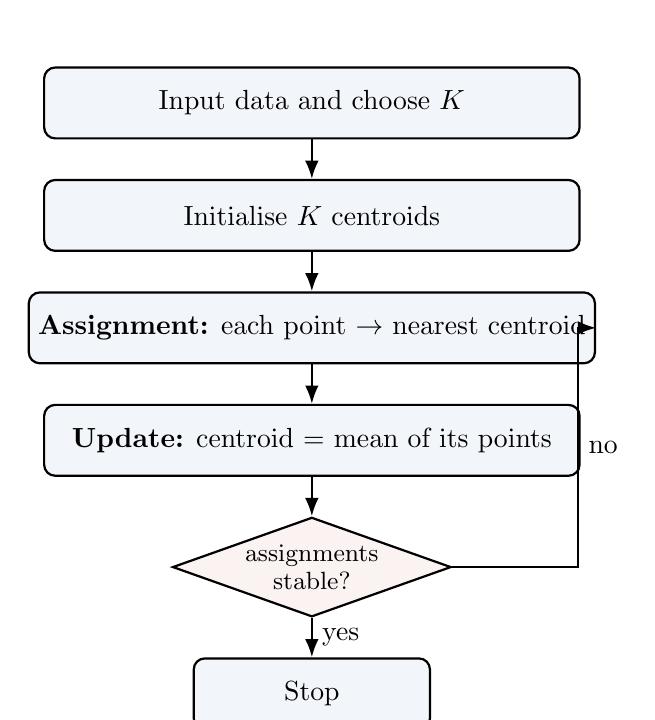
\begin{tikzpicture}[node distance=0.5cm,
  box/.style={draw,thick,rounded corners,align=center,minimum width=6.8cm,minimum height=9mm,fill=idea!6},
  dec/.style={draw,thick,diamond,aspect=2.8,align=center,fill=warn!6,inner sep=1pt}]
\node[box] (in) {Input data and choose $K$};
\node[box,below=of in] (init) {Initialise $K$ centroids};
\node[box,below=of init] (a) {\textbf{Assignment:} each point $\to$ nearest centroid};
\node[box,below=of a] (u) {\textbf{Update:} centroid $=$ mean of its points};
\node[dec,below=of u] (c) {\small assignments\\[-2pt]\small stable?};
\node[box,below=of c,minimum width=3cm] (s) {Stop};
\draw[-{Latex},thick] (in)--(init);
\draw[-{Latex},thick] (init)--(a);
\draw[-{Latex},thick] (a)--(u);
\draw[-{Latex},thick] (u)--(c);
\draw[-{Latex},thick] (c)--node[right]{yes}(s);
\draw[-{Latex},thick] (c.east)--++(1.6,0)|-node[pos=0.25,right]{no}(a.east);
\end{tikzpicture}
\end{center}

%======================================================================
\section{Complete Numerical Example}
%======================================================================

\textbf{Data:} eight examination marks, $X=\{45,50,55,70,75,80,90,95\}$, with $K=3$.

\subsection{Step 1: initialise}
\[
\mu_1^{(0)}=45,\qquad\mu_2^{(0)}=70,\qquad\mu_3^{(0)}=95.
\]
(These are illustrative starting values, conveniently placed; Section~\ref{sec:init} shows what happens with worse ones.)

\subsection{Step 2: distances and assignments}

\begin{center}
\begin{tabular}{@{}ccccc@{}}
\toprule
$x_n$ & $|x_n-45|$ & $|x_n-70|$ & $|x_n-95|$ & Assignment\\
\midrule
45 & \textbf{0} & 25 & 50 & $C_1$\\
50 & \textbf{5} & 20 & 45 & $C_1$\\
55 & \textbf{10} & 15 & 40 & $C_1$\\
70 & 25 & \textbf{0} & 25 & $C_2$\\
75 & 30 & \textbf{5} & 20 & $C_2$\\
80 & 35 & \textbf{10} & 15 & $C_2$\\
90 & 45 & 20 & \textbf{5} & $C_3$\\
95 & 50 & 25 & \textbf{0} & $C_3$\\
\bottomrule
\end{tabular}
\end{center}
\[
C_1=\{45,50,55\},\qquad C_2=\{70,75,80\},\qquad C_3=\{90,95\}.
\]
Note the mark $55$: it is $10$ from $\mu_1$ and $15$ from $\mu_2$, so it is the least certain member of $C_1$, but K-means records no such doubt.

\subsection{Step 3: update the centroids}
\[
\mu_1^{(1)}=\frac{45+50+55}{3}=50,\qquad
\mu_2^{(1)}=\frac{70+75+80}{3}=75,\qquad
\mu_3^{(1)}=\frac{90+95}{2}=92.5.
\]

\subsection{Step 4: repeat the assignment step}

\begin{center}
\begin{tabular}{@{}ccccc@{}}
\toprule
$x_n$ & $|x_n-50|$ & $|x_n-75|$ & $|x_n-92.5|$ & Assignment\\
\midrule
45 & \textbf{5} & 30 & 47.5 & $C_1$\\
50 & \textbf{0} & 25 & 42.5 & $C_1$\\
55 & \textbf{5} & 20 & 37.5 & $C_1$\\
70 & 20 & \textbf{5} & 22.5 & $C_2$\\
75 & 25 & \textbf{0} & 17.5 & $C_2$\\
80 & 30 & \textbf{5} & 12.5 & $C_2$\\
90 & 40 & 15 & \textbf{2.5} & $C_3$\\
95 & 45 & 20 & \textbf{2.5} & $C_3$\\
\bottomrule
\end{tabular}
\end{center}
No assignment changed, so recomputing the centroids gives the same values: the algorithm has \textbf{converged} after one update.

\begin{center}
\begin{tabular}{@{}lll@{}}
\toprule
Cluster & Observations & Centroid\\
\midrule
$C_1$ & 45, 50, 55 & 50\\
$C_2$ & 70, 75, 80 & 75\\
$C_3$ & 90, 95 & 92.5\\
\bottomrule
\end{tabular}
\end{center}

\begin{center}
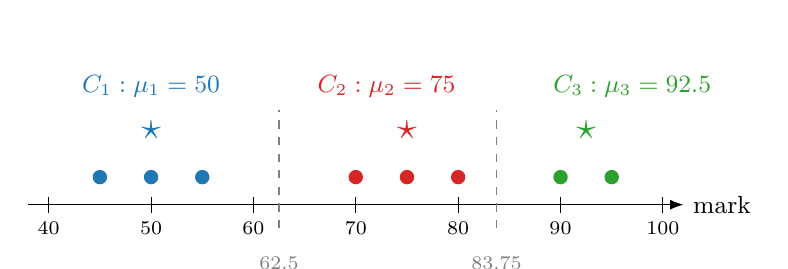
\begin{tikzpicture}[x=0.13cm]
\draw[-{Latex}] (38,0)--(102,0) node[right]{\small mark};
\foreach \t in {40,50,...,100}{\draw (\t,0.1)--(\t,-0.1) node[below,font=\scriptsize]{\t};}
\foreach \p in {45,50,55}{\fill[c1] (\p,0.35) circle (2.6pt);}
\foreach \p in {70,75,80}{\fill[c2] (\p,0.35) circle (2.6pt);}
\foreach \p in {90,95}{\fill[c3] (\p,0.35) circle (2.6pt);}
\node[c1,font=\Large] at (50,0.95) {$\star$};
\node[c2,font=\Large] at (75,0.95) {$\star$};
\node[c3,font=\Large] at (92.5,0.95) {$\star$};
\node[c1,font=\small] at (50,1.5) {$C_1:\mu_1=50$};
\node[c2,font=\small] at (73,1.5) {$C_2:\mu_2=75$};
\node[c3,font=\small] at (97,1.5) {$C_3:\mu_3=92.5$};
\draw[dashed,gray] (62.5,-0.3)--(62.5,1.2);
\draw[dashed,gray] (83.75,-0.3)--(83.75,1.2);
\node[gray,font=\scriptsize] at (62.5,-0.75) {62.5};
\node[gray,font=\scriptsize] at (83.75,-0.75) {83.75};
\end{tikzpicture}
\end{center}
Dashed lines are the \textbf{decision boundaries}, halfway between neighbouring centroids: $(50+75)/2=62.5$ and $(75+92.5)/2=83.75$. A new mark is classified simply by which interval it falls into.

\begin{example}[Example 4.1: A full 2-D run where a point changes cluster]
Six students (Maths, Physics):
$A=(40,45)$, $B=(45,50)$, $C=(50,40)$, $D=(80,85)$, $E=(85,80)$, $F=(90,90)$. Take $K=2$ and, deliberately, initial centroids $\mu_1=A=(40,45)$, $\mu_2=C=(50,40)$.

\textbf{Iteration 1, assignment} (squared distances):
\begin{center}
\begin{tabular}{@{}ccccccc@{}}
\toprule
& $A$ & $B$ & $C$ & $D$ & $E$ & $F$\\
\midrule
to $\mu_1=(40,45)$ & \textbf{0} & \textbf{50} & 125 & 3200 & 3250 & 4525\\
to $\mu_2=(50,40)$ & 125 & 125 & \textbf{0} & \textbf{2925} & \textbf{2825} & \textbf{4100}\\
\bottomrule
\end{tabular}
\end{center}
e.g.\ $\|D-\mu_2\|^2=(80-50)^2+(85-40)^2=900+2025=2925$. Clusters: $\{A,B\}$ and $\{C,D,E,F\}$.

\textbf{Update:} $\mu_1=(42.5,47.5)$, \quad $\mu_2=\big(\frac{50+80+85+90}{4},\frac{40+85+80+90}{4}\big)=(76.25,73.75)$.

\textbf{Iteration 2, assignment:} $\|C-\mu_1\|^2=7.5^2+7.5^2=112.5$ but $\|C-\mu_2\|^2=26.25^2+33.75^2=1828.1$, so $C$ \textbf{moves} to cluster 1. Clusters: $\{A,B,C\}$ and $\{D,E,F\}$.

\textbf{Update:} $\mu_1=(45,45)$, $\mu_2=(85,85)$. Iteration 3 changes nothing: converged.

The poor start put $C$ with the high scorers, but one update pulled $\mu_2$ far enough away to fix it.
\end{example}

%======================================================================
\section{The K-means Objective Function}
%======================================================================

K-means minimises the \textbf{within-cluster sum of squares} (WCSS), also called \emph{inertia}:
\[
\boxed{\;J=\sum_{k=1}^K\sum_{n:\,c_n=k}\|x_n-\mu_k\|^2,\qquad\min_{\{c_n\},\{\mu_k\}}J.\;}
\]
It measures how tightly each cluster hugs its centroid. Note that we optimise over two kinds of unknowns: the discrete labels $c_n$ and the continuous centroids $\mu_k$.

\begin{example}[Example 5.1: WCSS for the eight marks (handout example)]
\begin{align*}
J_1&=(45-50)^2+(50-50)^2+(55-50)^2=25+0+25=50,\\
J_2&=(70-75)^2+(75-75)^2+(80-75)^2=25+0+25=50,\\
J_3&=(90-92.5)^2+(95-92.5)^2=6.25+6.25=12.5,\\
J&=50+50+12.5=\mathbf{112.5}.
\end{align*}
\end{example}

\subsection{Why the algorithm always converges}

Each of the two steps can only lower (or keep) $J$:
\begin{itemize}[leftmargin=*]
\item \textbf{Assignment step} (centroids fixed): each term $\|x_n-\mu_{c_n}\|^2$ is minimised individually by choosing the nearest centroid.
\item \textbf{Update step} (labels fixed): for one cluster, $f(\mu)=\sum_{n\in C_k}(x_n-\mu)^2$ has derivative $-2\sum_{n\in C_k}(x_n-\mu)$, which is zero at the mean $\mu=\frac{1}{N_k}\sum_{n\in C_k}x_n$. So the mean is the best possible centre.
\end{itemize}
Since $J\ge0$ never increases and there are only finitely many ways to partition $N$ points, K-means must stop after a finite number of iterations. This is \emph{coordinate descent}, the hard-assignment twin of EM's coordinate ascent.

\begin{example}[Example 5.2: The mean is the best centre]
For $C_3=\{90,95\}$:
centre $92.5$: $2.5^2+2.5^2=12.5$; \quad centre $90$: $0^2+5^2=25$; \quad centre $95$: $25$; \quad centre $91$: $1+16=17$.
In general $\sum_n(x_n-c)^2=\sum_n(x_n-\bar x)^2+N_k(\bar x-c)^2$, so any centre other than the mean $\bar x$ pays an extra $N_k(\bar x-c)^2$. For $c=90$: $12.5+2(2.5)^2=25$. \checkmark
\end{example}

\subsection{Choosing \texorpdfstring{$K$}{K}: why WCSS alone fails, and the elbow}

WCSS always decreases as $K$ grows; with $K=N$ every point is its own centroid and $J=0$. So ``pick the $K$ with the smallest $J$'' always picks $K=N$. Instead, look for the \textbf{elbow}: the $K$ after which extra clusters give only small gains.

\begin{example}[Example 5.3: Best WCSS for each $K$ on the eight marks]
(For 1-D data the optimal clusters are contiguous runs of sorted values, so all splits can be checked.)
\begin{center}
\begin{tabular}{@{}clr@{}}
\toprule
$K$ & Best clustering & $J$\\
\midrule
1 & $\{45,\dots,95\}$ & 2400.0\\
2 & $\{45,50,55\}\ \{70,75,80,90,95\}$ & 480.0\\
3 & $\{45,50,55\}\ \{70,75,80\}\ \{90,95\}$ & 112.5\\
4 & $\{45\}\ \{50,55\}\ \{70,75,80\}\ \{90,95\}$ & 75.0\\
5 & $\{45\}\ \{50,55\}\ \{70\}\ \{75,80\}\ \{90,95\}$ & 37.5\\
8 & each point alone & 0.0\\
\bottomrule
\end{tabular}
\end{center}
\begin{center}
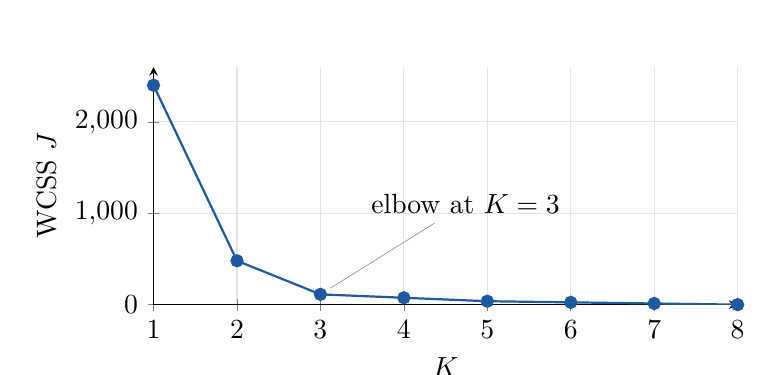
\begin{tikzpicture}
\begin{axis}[width=9cm,height=4.6cm,xlabel={$K$},ylabel={WCSS $J$},axis lines=left,xtick={1,...,8},
  ymin=0,ymax=2600,grid=major,grid style={gray!20},mark size=2pt]
\addplot[idea,thick,mark=*] coordinates {(1,2400) (2,480) (3,112.5) (4,75) (5,37.5) (6,25) (7,12.5) (8,0)};
\node[pin={[pin distance=0.9cm]60:{elbow at $K=3$}}] at (axis cs:3,112.5) {};
\end{axis}
\end{tikzpicture}
\end{center}
Going from $K=1\to2$ removes $1920$; $2\to3$ removes $367.5$; $3\to4$ removes only $37.5$. The curve bends at $K=3$, matching the three natural groups. For a less subjective choice, use the silhouette score, or fit a GMM and use BIC.
\end{example}

%======================================================================
\section{Limitations of K-means}
%======================================================================

\begin{center}
\renewcommand{\arraystretch}{1.2}
\begin{tabular}{@{}p{3.3cm}p{11.7cm}@{}}
\toprule
Limitation & Explanation\\
\midrule
Requires $K$ in advance & The number of clusters must be fixed before running.\\
Initialisation sensitivity & Different initial centroids may give different results; multiple starts or $k$-means++ help.\\
Outlier sensitivity & Extreme values pull centroids or grab whole clusters.\\
Cluster shape & Works best for compact, roughly spherical clusters of similar size and density.\\
Feature scaling & Features with large numerical ranges dominate the distance; standardisation may be needed.\\
Hard assignment & Each point gets one cluster; uncertainty in membership is not represented.\\
\bottomrule
\end{tabular}
\end{center}

\subsection{Initialisation sensitivity}\label{sec:init}

K-means converges, but only to a \emph{local} minimum of $J$.

\begin{example}[Example 6.1: Three different starts on the same eight marks]
\begin{center}
\begin{tabular}{@{}llcc@{}}
\toprule
Initial centroids & Final clusters & Iterations & Final $J$\\
\midrule
$(45,70,95)$ & $\{45,50,55\}\{70,75,80\}\{90,95\}$ & 2 & \textbf{112.5}\\
$(50,55,95)$ & $\{45,50,55\}\{70,75,80\}\{90,95\}$ & 4 & \textbf{112.5}\\
$(45,50,55)$ & $\{45\}\{50,55\}\{70,75,80,90,95\}$ & 3 & 442.5\\
\bottomrule
\end{tabular}
\end{center}
\textbf{Trace of the bad start $(45,50,55)$:}
\begin{itemize}[nosep]
\item Iteration 1: every mark from $55$ upwards is closest to the centroid $55$, so $C_1=\{45\}$, $C_2=\{50\}$, $C_3=\{55,70,\dots,95\}$. New centroids $(45,\ 50,\ 77.5)$, $J=1037.5$.
\item Iteration 2: $55$ is now closer to $50$, so $C_2=\{50,55\}$ and $C_3=\{70,\dots,95\}$. Centroids $(45,\ 52.5,\ 82)$, $J=442.5$.
\item Iteration 3: nothing changes. Stuck.
\end{itemize}
Two centroids were ``wasted'' on the low group, and the high group never got split. $J=442.5$ is almost $4\times$ worse than the best $112.5$, yet no single assignment or update step can improve it.

\textbf{Remedy:} run K-means several times (e.g.\ 10 restarts) and keep the run with the smallest $J$; or use $k$-means++.
\end{example}

\subsection{\texorpdfstring{$k$}{k}-means++ initialisation}\label{sec:kpp}

$k$-means++ spreads the initial centroids out: pick the first centroid uniformly at random; then pick each next centroid from the data with probability proportional to $D(x)^2$, the squared distance to the nearest centroid already chosen.

\begin{example}[Example 6.2: $k$-means++ second-centroid probabilities]
Suppose the first centroid is $45$. Then $D(x)^2=(x-45)^2$:
\begin{center}
\begin{tabular}{@{}lcccccccc@{}}
\toprule
$x$ & 45 & 50 & 55 & 70 & 75 & 80 & 90 & 95\\
\midrule
$D(x)^2$ & 0 & 25 & 100 & 625 & 900 & 1225 & 2025 & 2500\\
$P(\text{pick }x)$ & 0 & 0.003 & 0.014 & 0.084 & 0.122 & 0.166 & 0.274 & 0.338\\
\bottomrule
\end{tabular}
\end{center}
(Sum of $D^2$ is $7400$; e.g.\ $P(95)=2500/7400=0.338$.) There is a $61\%$ chance the second centroid lands in the top group $\{90,95\}$ and only a $1.7\%$ chance it lands near $45$ again, which avoids the bad start of Example 6.1.
\end{example}

\subsection{Outlier sensitivity}

\begin{example}[Example 6.3: One typo of 300]
Add an erroneous mark $300$ to the data and rerun from $(45,70,95)$:
\begin{itemize}[nosep]
\item Iteration 1: $300\to C_3$, so $\mu_3=\frac{90+95+300}{3}=161.7$, far from every real mark.
\item Iteration 2: $90$ and $95$ are now closer to $75$ than to $161.7$, so they join $C_2$. The outlier keeps $C_3$ to itself: $\mu_3=300$.
\end{itemize}
Final clusters: $\{45,50,55\}$, $\{70,75,80,90,95\}$, $\{300\}$. One bad value \emph{used up a whole cluster} and merged two real groups. Remedies: clean the data, detect outliers first, or use $k$-medoids (centres must be actual data points; less sensitive).
\end{example}

\subsection{Feature scaling}

\begin{example}[Example 6.4: Age and income]
Three people: $P_1=(25\text{ yrs},\ 50{,}000)$, $P_2=(60\text{ yrs},\ 51{,}000)$, $P_3=(27\text{ yrs},\ 58{,}000)$ (income in Taka per month).

\textbf{Raw distances:}
$d(P_1,P_2)=\sqrt{35^2+1000^2}\approx1000.6$, \quad $d(P_1,P_3)=\sqrt{2^2+8000^2}\approx8000.0$.
So $P_1$ looks closest to the 60-year-old: income differences of thousands swamp an age gap of 35 years.

\textbf{After min--max scaling} with ages in $[20,70]$ and incomes in $[20{,}000,\,120{,}000]$, i.e.\ $x'=(x-\min)/(\max-\min)$:
$P_1'=(0.10,\,0.30)$, $P_2'=(0.80,\,0.31)$, $P_3'=(0.14,\,0.38)$.
\[
d(P_1',P_2')=\sqrt{0.70^2+0.01^2}\approx0.700,\qquad d(P_1',P_3')=\sqrt{0.04^2+0.08^2}\approx0.089.
\]
Now $P_1$ is clearly closest to $P_3$ (similar age \emph{and} similar income). Always put features on comparable scales (min--max or $z$-score standardisation) before K-means.
\end{example}

\subsection{Cluster shape}

K-means boundaries are straight lines halfway between centroids, and it implicitly assumes every cluster is a similarly sized round blob. It fails on elongated, curved (e.g.\ two interleaved crescents) or very unequal clusters: a big, wide cluster gets split while a nearby small one gets absorbed. GMMs (with their own covariance per component) handle elliptical clusters; spectral or density-based methods (DBSCAN) handle curved ones.

%======================================================================
\section{K-means and Gaussian Mixture Models}\label{sec:gmm}
%======================================================================

\begin{center}
\renewcommand{\arraystretch}{1.15}
\begin{tabular}{@{}p{3.6cm}p{5cm}p{5.8cm}@{}}
\toprule
Feature & K-means & GMM using EM\\
\midrule
Cluster representation & Centroid & Gaussian distribution\\
Assignment & Nearest centroid & Posterior responsibility $r_{nk}$\\
Membership & Hard (0 or 1) & Soft ($0\le r_{nk}\le1$)\\
Mean update & Arithmetic mean & Responsibility-weighted mean\\
Extra parameters & None (no variance model) & Mixing probabilities and covariances\\
Objective & Minimise WCSS & Maximise data log-likelihood\\
Can generate data? & No & Yes (sample from the fitted mixture)\\
\bottomrule
\end{tabular}
\end{center}

\subsection{From soft assignment to hard assignment}

In a GMM the E-step computes responsibilities
\[
r_{nk}=\frac{\pi_k\,\N(x_n\mid\mu_k,\Sigma_k)}{\sum_{j=1}^K\pi_j\,\N(x_n\mid\mu_j,\Sigma_j)}.
\]
Now make every component the same shape: $\pi_k=1/K$ and $\Sigma_k=\sigma^2I$. The weights and normalising constants are identical for every $k$, so they cancel and
\[
r_{nk}\propto\exp\!\left(-\frac{\|x_n-\mu_k\|^2}{2\sigma^2}\right).
\]
Comparing any other component $j$ with the nearest one $k$:
\[
\frac{r_{nj}}{r_{nk}}=\exp\!\left(-\frac{\|x_n-\mu_j\|^2-\|x_n-\mu_k\|^2}{2\sigma^2}\right)\xrightarrow{\ \sigma^2\to0\ }0,
\]
because the numerator in the exponent is positive. Hence, \emph{provided the nearest centroid is unique},
\[
r_{nk}\to\begin{cases}1,&k=\argmin_j\|x_n-\mu_j\|^2,\\0,&\text{otherwise,}\end{cases}
\qquad\text{and}\qquad
\mu_k=\frac{\sum_nr_{nk}x_n}{\sum_nr_{nk}}\;\to\;\frac{1}{N_k}\sum_{n:\,c_n=k}x_n .
\]
The E-step becomes the K-means assignment step and the M-step becomes the K-means update. \textbf{K-means is the limit of GMM-EM with equal weights, equal spherical covariances and $\sigma^2\to0$.}

\begin{example}[Example 7.1: Watching responsibilities harden]
Use the final centroids $(50,\,75,\,92.5)$, equal weights, and shrink the common variance.
\begin{center}
\begin{tabular}{@{}lcccc@{}}
\toprule
& $\sigma^2=100$ & $\sigma^2=25$ & $\sigma^2=4$ & $\sigma^2=1$\\
\midrule
$x=60$: $(r_1,r_2,r_3)$ & $(0.648,\,0.347,\,0.005)$ & $(0.924,\,0.076,\,0)$ & $(1,\,0,\,0)$ & $(1,\,0,\,0)$\\
$x=62.5$: $(r_1,r_2,r_3)$ & $(0.494,\,0.494,\,0.012)$ & $(0.5,\,0.5,\,0)$ & $(0.5,\,0.5,\,0)$ & $(0.5,\,0.5,\,0)$\\
\bottomrule
\end{tabular}
\end{center}
\textbf{Worked entry} ($x=60$, $\sigma^2=25$): exponents $-\frac{10^2}{50}=-2$, $-\frac{15^2}{50}=-4.5$, $-\frac{32.5^2}{50}=-21.1$, so
$r_1=\dfrac{e^{-2}}{e^{-2}+e^{-4.5}+e^{-21.1}}=\dfrac{0.1353}{0.1353+0.0111}=0.924$.

For $x=60$ (nearest centroid $50$ is unique) the responsibilities snap to the K-means answer. For $x=62.5$, exactly on the boundary, they stay at $0.5/0.5$ however small $\sigma^2$ gets. That is why the handout's statement needs the qualification ``provided there is a unique nearest centroid''.
\end{example}

\begin{caution}[Zero variance is a limit, not a substitution]
A Gaussian with $\sigma^2=0$ is not a proper density (it is an infinitely tall spike). The connection is a \emph{limiting} argument: we study what happens as $\sigma^2$ gets smaller and smaller, never at $\sigma^2=0$ itself.
\end{caution}

\begin{example}[Example 7.2: Turning the K-means result into a generative GMM]
K-means cannot create new data, but its clusters give a good GMM starting point. From the final clusters:
\begin{center}
\begin{tabular}{@{}lccc@{}}
\toprule
& $\pi_k=N_k/N$ & $\mu_k$ & $\sigma_k^2=J_k/N_k$\\
\midrule
Component 1 & $3/8=0.375$ & 50 & $50/3=16.67$\\
Component 2 & $3/8=0.375$ & 75 & $50/3=16.67$\\
Component 3 & $2/8=0.250$ & 92.5 & $12.5/2=6.25$\\
\bottomrule
\end{tabular}
\end{center}
\textbf{Generate a new mark:} draw $u=0.81$; cumulative weights are $0.375,\,0.75,\,1$, so choose component 3. Draw $\epsilon=-0.6$ from $\N(0,1)$: $x=92.5+\sqrt{6.25}\,(-0.6)=92.5-1.5=91.0$. This is a new student mark that was never in the data, which is exactly what a generative model does. (This GMM is also a good initialisation for EM.)
\end{example}

%======================================================================
\section{K-means and Generative AI}
%======================================================================

\textbf{K-means is not itself a generative model.} It groups observations; a generative model learns a probability distribution (or a sampling procedure) and uses it to produce new samples. But the core K-means operation, \emph{replace a vector by its nearest prototype}, reappears inside modern generative systems.

\begin{center}
\renewcommand{\arraystretch}{1.15}
\begin{tabular}{@{}p{3.2cm}p{5.4cm}p{6.2cm}@{}}
\toprule
Aspect & K-means & Generative AI\\
\midrule
Main purpose & Group similar observations & Learn data patterns and generate new samples\\
Output & Cluster labels and centroids & New text, images, audio or other data\\
Typical objective & Minimise within-cluster squared distance & Model-dependent: likelihood, ELBO, adversarial loss, \dots\\
Generates new samples? & Not by itself & Yes, by design\\
\bottomrule
\end{tabular}
\end{center}

%======================================================================
\section{Application 1: Clustering Latent Representations}
%======================================================================

A neural encoder maps an input (an image, a sentence) to an \textbf{embedding} or latent vector:
\[
x\ \xrightarrow{\text{Encoder}}\ z,\qquad z\in\mathbb{R}^D.
\]
After embedding many inputs, K-means groups similar embeddings:
\[
\{z_1,\dots,z_N\}\xrightarrow{\text{K-means}}\{C_1,\dots,C_K\}.
\]

\begin{center}
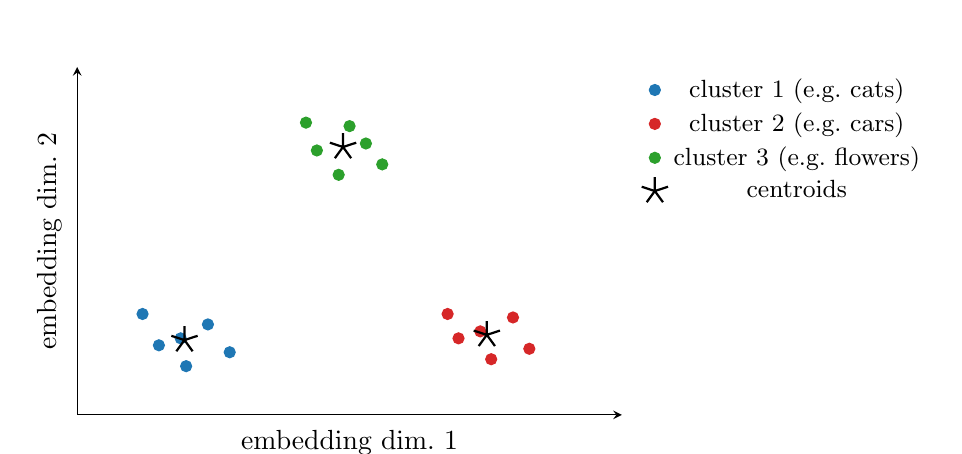
\begin{tikzpicture}
\begin{axis}[width=8.5cm,height=6cm,xlabel={embedding dim.\ 1},ylabel={embedding dim.\ 2},
  axis lines=left,xmin=0,xmax=10,ymin=0,ymax=10,xtick=\empty,ytick=\empty,
  legend style={font=\small,draw=none,at={(1.02,1)},anchor=north west}]
\addplot[only marks,mark=*,c1,mark size=2pt] coordinates {(1.5,2) (2,1.4) (2.4,2.6) (1.2,2.9) (2.8,1.8) (1.9,2.2)};
\addplot[only marks,mark=*,c2,mark size=2pt] coordinates {(7,2.2) (7.6,1.6) (8,2.8) (6.8,2.9) (7.4,2.4) (8.3,1.9)};
\addplot[only marks,mark=*,c3,mark size=2pt] coordinates {(4.4,7.6) (5,8.3) (5.6,7.2) (4.8,6.9) (5.3,7.8) (4.2,8.4)};
\addplot[only marks,mark=star,black,mark size=5pt,thick] coordinates {(1.97,2.15) (7.52,2.3) (4.88,7.7)};
\legend{{cluster 1 (e.g.\ cats)},{cluster 2 (e.g.\ cars)},{cluster 3 (e.g.\ flowers)},{centroids}}
\end{axis}
\end{tikzpicture}
\end{center}
This is a schematic 2-D picture of a high-dimensional space. \textbf{K-means does not understand images}: it only measures distances. The clusters are meaningful only if the encoder has placed semantically similar inputs close together.

\begin{example}[Example 9.1: Cosine vs.\ Euclidean distance for embeddings]
Embeddings are often compared by direction rather than length. Take $z_a=(2,0)$, $z_b=(10,0)$, $z_c=(1.5,1.5)$. Euclidean: $\|z_a-z_b\|=8$, $\|z_a-z_c\|=\sqrt{0.25+2.25}=1.58$, so $z_a$ looks closest to $z_c$. Cosine similarity: $\cos(z_a,z_b)=1$ (same direction) but $\cos(z_a,z_c)=\frac{3}{2\cdot2.121}=0.707$. A common fix is to \textbf{L2-normalise} embeddings ($z/\|z\|$) before K-means; then squared Euclidean distance equals $2-2\cos$, and both views agree.
\end{example}

%======================================================================
\section{Application 2: Vector Quantization and VQ-VAE}
%======================================================================

\subsection{The idea}

A \textbf{Vector-Quantised Variational Autoencoder} (VQ-VAE) has an encoder, a discrete \textbf{codebook} and a decoder.
\begin{align*}
&\text{Encoder:} && z_e(x)=\mathrm{Encoder}(x)\\
&\text{Codebook:} && E=\{e_1,e_2,\dots,e_K\}\quad(\text{$K$ learned vectors})\\
&\text{Quantise:} && k^\ast=\argmin_k\|z_e(x)-e_k\|_2^2,\qquad z_q(x)=e_{k^\ast}\\
&\text{Decoder:} && \hat x=\mathrm{Decoder}(z_q(x))
\end{align*}
The quantise step is \emph{exactly} the K-means assignment step, with codebook vectors playing the role of centroids. The difference: the codebook is learned \emph{jointly} with the encoder and decoder by gradient descent, not by running K-means once on fixed data.

\begin{center}
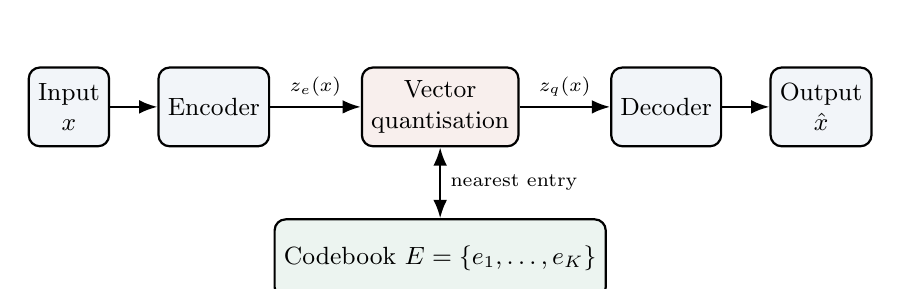
\begin{tikzpicture}[node distance=1.15cm,
  b/.style={draw,thick,rounded corners,align=center,minimum height=10mm,fill=idea!6,font=\small}]
\node[b] (x) {Input\\$x$};
\node[b,right=0.6cm of x] (enc) {Encoder};
\node[b,right=of enc,fill=warn!8] (vq) {Vector\\quantisation};
\node[b,right=of vq] (dec) {Decoder};
\node[b,right=0.6cm of dec] (xh) {Output\\$\hat x$};
\node[b,below=0.9cm of vq,fill=exam!8] (cb) {Codebook $E=\{e_1,\dots,e_K\}$};
\draw[-{Latex},thick] (x)--(enc);
\draw[-{Latex},thick] (enc)--node[above,font=\scriptsize]{$z_e(x)$}(vq);
\draw[-{Latex},thick] (vq)--node[above,font=\scriptsize]{$z_q(x)$}(dec);
\draw[-{Latex},thick] (dec)--(xh);
\draw[{Latex}-{Latex},thick] (cb)--node[right,font=\scriptsize]{nearest entry}(vq);
\end{tikzpicture}
\end{center}

\begin{example}[Example 10.1: Selecting the nearest codebook vector (handout example)]
Encoder output $z_e(x)=(3,4)$; codebook $e_1=(1,2)$, $e_2=(4,5)$, $e_3=(8,8)$.
\begin{align*}
d_1^2&=(3-1)^2+(4-2)^2=4+4=8,\\
d_2^2&=(3-4)^2+(4-5)^2=1+1=2,\\
d_3^2&=(3-8)^2+(4-8)^2=25+16=41.
\end{align*}
The smallest is $d_2^2=2$, so $k^\ast=2$ and $z_q(x)=e_2=(4,5)$. The continuous vector $(3,4)$ is replaced by the discrete \textbf{token} ``2''. Only the index needs to be stored or modelled.
\end{example}

\subsection{How the codebook is trained}

The quantisation step $\argmin$ has no useful gradient, so VQ-VAE uses three tricks.

\textbf{1. Straight-through estimator.} In the backward pass, the gradient arriving at $z_q$ is copied directly to $z_e$, as if quantisation were the identity. This lets the encoder learn.

\textbf{2. Loss with three terms} ($\sg[\cdot]$ = stop-gradient, i.e.\ treat as a constant):
\[
\mathcal{L}=\underbrace{\|x-\hat x\|^2}_{\text{reconstruction}}
+\underbrace{\|\sg[z_e(x)]-e_{k^\ast}\|^2}_{\text{codebook loss: move }e\text{ towards }z_e}
+\beta\underbrace{\|z_e(x)-\sg[e_{k^\ast}]\|^2}_{\text{commitment: keep }z_e\text{ near }e},
\]
with $\beta$ typically $0.25$.

\textbf{3. Or a K-means-style update.} Many implementations replace the codebook loss by an exponential moving average: each $e_k$ is moved towards the \emph{mean} of the encoder vectors assigned to it. That is literally a (smoothed) K-means update step.

\begin{example}[Example 10.2: Codebook loss and updates for the same vector]
With $z_e=(3,4)$, $e_{k^\ast}=e_2=(4,5)$ and $\beta=0.25$:
\[
\text{codebook loss}=\|(3,4)-(4,5)\|^2=2,\qquad\text{commitment loss}=0.25\times2=0.5.
\]
\textbf{Gradient step on $e_2$} (learning rate $\eta=0.1$): $\nabla_{e_2}\|z_e-e_2\|^2=-2(z_e-e_2)=(2,2)$, so
$e_2\leftarrow(4,5)-0.1(2,2)=(3.8,\,4.8)$: the code vector moves towards the encoder output.

\textbf{K-means-style update:} suppose a mini-batch produces encoder vectors $(3,4)$, $(5,6)$ and $(4,4)$. Check: $(5,6)$ has $d^2=(32,\ 2,\ 13)$ and $(4,4)$ has $d^2=(13,\ 1,\ 32)$ to $(e_1,e_2,e_3)$, so all three choose $e_2$. The K-means update sets
$e_2\leftarrow\big(\tfrac{3+5+4}{3},\tfrac{4+6+4}{3}\big)=(4,\ 4.67)$, the centroid of its assigned vectors.
\end{example}

\subsection{How VQ-VAE generates new data}

Training gives a \emph{discrete} representation: an image becomes a grid of codebook indices. To generate:
\begin{enumerate}[nosep]
\item Train a \textbf{prior} over index grids or sequences (originally PixelCNN; now usually a Transformer that predicts the next token).
\item Sample a new grid of indices from the prior.
\item Look up each index in the codebook and run the decoder to get a brand-new image.
\end{enumerate}
This is how continuous data (images, audio, video) can be modelled with the same next-token machinery as text.

\begin{example}[Example 10.3: How much does tokenisation compress?]
An illustrative setup: a $256\times256$ RGB image is encoded to a $32\times32$ grid of codes, with a codebook of $K=512$ entries.
\begin{itemize}[nosep]
\item Raw image: $256\times256\times3=196{,}608$ bytes.
\item Codes: $32\times32=1024$ indices, each needing $\log_2512=9$ bits: $1024\times9=9216$ bits $=1152$ bytes.
\end{itemize}
About $170\times$ smaller, and the prior now models a sequence of only $1024$ tokens instead of $196{,}608$ pixel values. (The decoder must reconstruct fine detail, so quality depends on how good the codebook and decoder are.)
\end{example}

\subsection{Applications of VQ-VAE}

\begin{itemize}[nosep]
\item \textbf{Image generation and compression:} images become discrete visual tokens; Transformers generate new token grids; storage is a compact index grid.
\item \textbf{Audio, speech and music:} waveforms or audio features become tokens for speech synthesis and music generation.
\item \textbf{Video:} spatio-temporal tokens for prediction and generation.
\item \textbf{Robotics and medical imaging:} compact representations of sensor data, actions or scans for reconstruction and generative modelling.
\item \textbf{Generative AI with Transformers:} any continuous signal becomes a sequence of integers, so ``predict the next token'' applies.
\item \textbf{Representation learning:} a finite vocabulary of useful latent patterns for downstream tasks.
\item \textbf{Connection with K-means:} nearest-codebook assignment is nearest-centroid assignment, but the codebook is learned inside the encoder--decoder.
\end{itemize}

%======================================================================
\section{Application 3: Dataset Organisation}
%======================================================================

Before training a generative model, K-means on embeddings is a cheap way to inspect a large dataset:
\begin{enumerate}[nosep]
\item Extract embeddings for every item.
\item Run K-means on the embeddings.
\item Inspect each cluster and a few representative samples (those nearest the centroid).
\item Spot near-duplicates (tiny, very tight clusters), unusual or junk groups, and under-represented regions.
\item Use this to guide curation: deduplicate, remove junk, or re-balance sampling.
\end{enumerate}

\begin{example}[Example 11.1: Re-balancing a Bangla text corpus]
Suppose $100{,}000$ Bangla documents are clustered into $K=4$ topics with sizes $70{,}000$ (news), $20{,}000$ (social media), $8{,}000$ (literature) and $2{,}000$ (science). Sampling uniformly, the model sees science only $2\%$ of the time. Sampling uniformly \emph{per cluster} (each cluster $25\%$) raises science to $25\%$, so each science document is seen $\frac{0.25}{0.02}=12.5\times$ more often. Whether this helps depends on the goal (and repeated small clusters risk overfitting); clustering only \emph{informs} the decision.
\end{example}
Clustering alone does not guarantee a better generative model; it is an analysis tool.

%======================================================================
\section{Conceptual Connection: Mixture-of-Experts}
%======================================================================

A \textbf{Mixture-of-Experts} (MoE) model has several expert networks $f_1,\dots,f_K$ and a learned \textbf{router} (gate) $g$ that decides how much each expert contributes:
\[
y=\sum_{k=1}^Kg_k(x)\,f_k(x),\qquad g_k(x)\ge0,\quad\sum_{k=1}^Kg_k(x)=1.
\]
The router usually produces scores $s_k(x)$ and normalises them with a softmax:
\[
g_k(x)=\frac{\exp(s_k(x))}{\sum_{j=1}^K\exp(s_j(x))}.
\]

\begin{center}
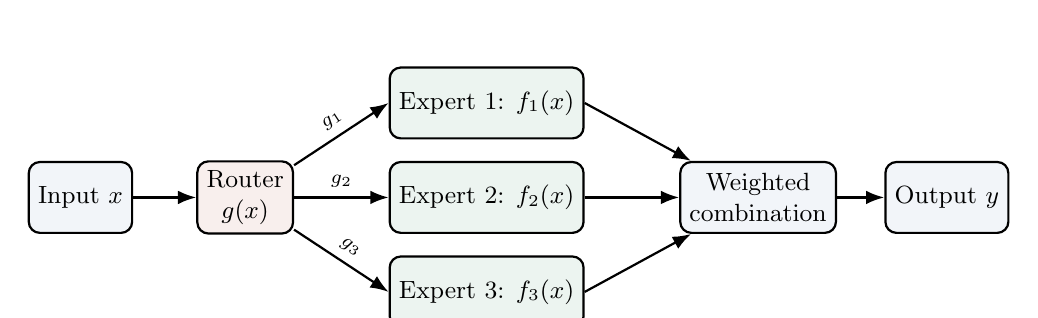
\begin{tikzpicture}[node distance=0.5cm,
  b/.style={draw,thick,rounded corners,align=center,minimum height=9mm,font=\small,fill=idea!6}]
\node[b] (x) {Input $x$};
\node[b,right=0.8cm of x,fill=warn!8] (r) {Router\\$g(x)$};
\node[b,right=1.2cm of r,yshift=1.2cm,fill=exam!8] (e1) {Expert 1: $f_1(x)$};
\node[b,right=1.2cm of r,fill=exam!8] (e2) {Expert 2: $f_2(x)$};
\node[b,right=1.2cm of r,yshift=-1.2cm,fill=exam!8] (e3) {Expert 3: $f_3(x)$};
\node[b,right=1.2cm of e2] (c) {Weighted\\combination};
\node[b,right=0.6cm of c] (y) {Output $y$};
\draw[-{Latex},thick] (x)--(r);
\foreach \e/\w in {e1/g_1,e2/g_2,e3/g_3}{\draw[-{Latex},thick] (r)--node[above,font=\scriptsize,sloped]{$\w$}(\e.west); \draw[-{Latex},thick] (\e.east)--(c);}
\draw[-{Latex},thick] (c)--(y);
\end{tikzpicture}
\end{center}

\begin{example}[Example 12.1: Dense MoE (handout example)]
Experts: Mathematics, Physics, Chemistry. Router weights $g(x)=(0.70,\,0.20,\,0.10)$; expert outputs $f(x)=(80,\,60,\,90)$.
\[
y=0.70(80)+0.20(60)+0.10(90)=56+12+9=\mathbf{77}.
\]
The answer leans towards the Mathematics expert because the router trusts it most for this input.
\end{example}

\begin{example}[Example 12.2: Where the router weights come from]
Suppose the router's scores are $s(x)=(2.0,\,0.75,\,0.05)$.
\[
e^{2.0}=7.389,\quad e^{0.75}=2.117,\quad e^{0.05}=1.051,\quad\text{sum}=10.557,
\]
\[
g(x)=\Big(\tfrac{7.389}{10.557},\ \tfrac{2.117}{10.557},\ \tfrac{1.051}{10.557}\Big)=(0.700,\ 0.201,\ 0.100),
\]
which reproduces the weights of Example 12.1. Softmax guarantees the weights are positive and sum to one.
\end{example}

\begin{example}[Example 12.3: Sparse (top-$k$) routing]
Large MoE language models run only the top one or two experts per token to save computation, then renormalise.

\textbf{Top-2:} keep Maths and Physics, renormalise $0.70/0.90=0.778$ and $0.20/0.90=0.222$:
$y=0.778(80)+0.222(60)=62.2+13.3=\mathbf{75.6}$.

\textbf{Top-1:} only Maths runs: $y=80$.

With, say, 8 experts and top-2 routing, each token uses only $2/8=25\%$ of the expert computation, while the model still has the capacity (parameters) of all 8. Training usually adds a \emph{load-balancing} loss so the router does not send everything to one favourite expert.
\end{example}

\textbf{Relation to K-means.} Top-1 routing resembles a hard cluster assignment (each input goes to one specialist), and dense routing resembles soft GMM responsibilities. But the router is a \emph{learned neural network} trained end-to-end for the task, not K-means, and it may select several experts per input.

%======================================================================
\section{Comparison: K-means, GMM, VQ-VAE and MoE}
%======================================================================

\begin{center}
\renewcommand{\arraystretch}{1.2}
\small
\begin{tabular}{@{}p{2.4cm}p{2.7cm}p{3cm}p{3.1cm}p{3.3cm}@{}}
\toprule
Feature & K-means & GMM & VQ-VAE & MoE\\
\midrule
Main purpose & Clustering & Probabilistic clustering / density model & Generative modelling & Conditional computation\\
Representation & Centroids & Gaussian components & Learned codebook vectors & Expert networks\\
Assignment & Hard (nearest centroid) & Soft (responsibilities) & Hard (nearest code) & Learned router (soft or top-$k$)\\
Probability model & No explicit density & Yes & Learned prior over codes $+$ decoder & Router weights only\\
Generates new content? & No, not by itself & Can sample from the fitted mixture & Yes (prior $+$ decoder) & Not by itself; depends on the overall model\\
Trained by & Alternating assign/update & EM & Gradient descent ($+$ straight-through) & Gradient descent\\
\bottomrule
\end{tabular}
\end{center}

%======================================================================
\section{Summary and Learning Progression}
%======================================================================

\begin{enumerate}[nosep]
\item K-means alternates nearest-centroid assignment and mean updates; it minimises WCSS and always converges, but only to a local minimum.
\item It needs $K$ in advance, is sensitive to initialisation, outliers and feature scales, and gives hard assignments.
\item K-means is the $\sigma^2\to0$ limit of GMM-EM with equal weights and equal spherical covariances.
\item K-means is a clustering algorithm, not a generative model by itself, but it can organise learned embeddings and datasets.
\item Nearest-centroid assignment is the quantisation step of VQ-VAE, whose learned codebook turns continuous representations into discrete tokens that a prior can generate.
\item Mixture-of-Experts uses a learned router to spread computation over experts; it is conceptually related to grouping, but it is not K-means.
\end{enumerate}

\begin{center}
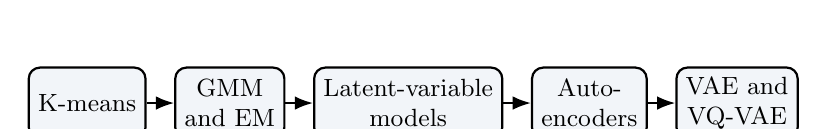
\begin{tikzpicture}[node distance=0.35cm,b/.style={draw,thick,rounded corners,align=center,font=\small,fill=idea!6,minimum height=9mm}]
\node[b] (a) {K-means};
\node[b,right=of a] (b) {GMM\\and EM};
\node[b,right=of b] (c) {Latent-variable\\models};
\node[b,right=of c] (d) {Auto-\\encoders};
\node[b,right=of d] (e) {VAE and\\VQ-VAE};
\foreach \u/\v in {a/b,b/c,c/d,d/e}{\draw[-{Latex},thick] (\u)--(\v);}
\end{tikzpicture}
\end{center}
Each step adds one idea: soft probabilistic assignment (GMM), hidden variables and EM (latent-variable models), learned neural encoders (autoencoders), and finally probabilistic or discrete latent spaces that can be \emph{sampled} to generate new data (VAE, VQ-VAE).

%======================================================================
\section{Formula Sheet and Practice}
%======================================================================

\begin{center}
\renewcommand{\arraystretch}{1.5}
\begin{tabular}{@{}ll@{}}
\toprule
Centroid & $\mu_k=\frac{1}{N_k}\sum_{x_n\in C_k}x_n$\\
Euclidean distance & $\|x_n-\mu_k\|=\sqrt{\sum_j(x_{nj}-\mu_{kj})^2}$\\
Assignment & $c_n=\argmin_k\|x_n-\mu_k\|^2$\\
WCSS objective & $J=\sum_k\sum_{n:c_n=k}\|x_n-\mu_k\|^2$\\
Mean is optimal & $\sum_n(x_n-c)^2=\sum_n(x_n-\bar x)^2+N(\bar x-c)^2$\\
$k$-means++ & $P(\text{next centre}=x)\propto D(x)^2$\\
GMM $\to$ K-means & $r_{nk}\propto\exp(-\|x_n-\mu_k\|^2/2\sigma^2)\to$ hard as $\sigma^2\to0$\\
VQ & $k^\ast=\argmin_k\|z_e(x)-e_k\|^2$, \quad $z_q(x)=e_{k^\ast}$\\
VQ-VAE loss & $\|x-\hat x\|^2+\|\sg[z_e]-e_{k^\ast}\|^2+\beta\|z_e-\sg[e_{k^\ast}]\|^2$\\
MoE & $y=\sum_kg_k(x)f_k(x)$, \quad $g_k=\mathrm{softmax}(s)_k$\\
\bottomrule
\end{tabular}
\end{center}

\subsection*{Practice questions}
\begin{enumerate}
\item With the final centroids $(50,\,75,\,92.5)$, which cluster does a new mark of $62$ join?
\item If the mark $70$ were forced into cluster 1 (centroids recomputed), what would the total WCSS be?
\item With the codebook of Example 10.1, which code does $z_e=(7,6)$ map to?
\item An MoE router gives $g=(0.5,\,0.3,\,0.2)$ with expert outputs $(80,\,60,\,90)$. Find $y$, and $y$ under top-1 routing.
\item Why can't WCSS alone be used to choose $K$?
\end{enumerate}

\textbf{Answers.}
\begin{enumerate}
\item Distances $12,\ 13,\ 30.5$, so $C_1$. (It is just below the boundary $62.5$.)
\item $C_1=\{45,50,55,70\}$ has mean $55$ and $J_1=100+25+0+225=350$; $C_2=\{75,80\}$ has mean $77.5$ and $J_2=12.5$; $J_3=12.5$. Total $375$, much worse than $112.5$.
\item $d^2=(36+16,\ 9+1,\ 1+4)=(52,\ 10,\ 5)$, so $e_3=(8,8)$.
\item $y=40+18+18=76$; top-1 keeps only expert 1, so $y=80$.
\item WCSS always decreases as $K$ increases (it is $0$ at $K=N$), so it would always choose the largest $K$. Use the elbow, silhouette, or a likelihood-based criterion such as BIC.
\end{enumerate}

\end{document}
